
\chapter{基于海量路由数据的图网络生成算法}

% 8-10 页

% 0.3 页
目前已经有一些网络研究机构和组织提供了自己收集的全球路由表数据集,并且已经在部分路由异常检测的研究中使用。然而这些数据集并不是图网络数据集,存在一些对于图网络而言不易处理的特征,因而大多数研究并非通过图的角度出发,而是简单地将这些数据集理解为路由更新时间序列,从而损失了其中携带的拓扑信息。因此,为了探索在现有路由数据上进行图的构造,进而将路由异常问题转化为完全可由典型图网络模型处理的图数据,本研究结合路由数据的特点,构建了一种图网络数据集生成算法,并通过一些公开可用的网络路由数据集提取出了相应的图网络数据。

\section{研究背景}

% 2 页

\subsection{现有的网络路由数据集}

现有的互联网络路由数据集通常是由中立机构收集和发布的,借助分布式的收集系统和路由反馈会话,此类机构能够从互联网上不同的位置收集全球路由表中的实时 BGP 信息,并将其制作为格式化的数据库进行发布。

由于 BGP 路由条目是以路径的形式呈现,从单个或少数几个自治系统的路由表中获得的路由信息是极为有限的,同时由于最短路径原则在路径上的体现是一类最小/次小生成树结构的叠加,据此构建的图样本将以采样中心呈现类树状结构,不具有普通性,也不是本研究的研究目标。因此,本文只关注以下具有更加广泛的收集覆盖面的数据集。

RIPE RIS 是路由异常分析中一个最常见的路由数据来源,它由若干位于互联网交换中心的远程路由收集器(RRC) 收集和存储来自参与者通过 BGP 提供的路由数据,其中包含了来自数十个国家的上万个自治系统收集的路由信息。一些路由异常预警系统采用了由该项目反馈的实时数据\citing{ripe2021routing}。

RoutesView 项目\citing{denardis2020internet}是另一个类似的大型数据采集工程,它从 1997 年以来不断收集和归档全球互联网路由表的每日快照,并在全球各地与不同规模的网络建立了 BGP 路由收集会话。

几乎所有可用的网络路由数据都使用 MRT 格式\citing{blunk2011multi},它能够完整地记录路由表中的多种路由信息,其中自治系统路径是表现拓扑结构的主要信息,而社区属性则反映了路由的优先级。

\subsection{现有数据集在图网络算法中的不足}

由于现有的数据集大多以 MRT 数据集提供,此类数据集本身是一类随机事件流,不是现成的图数据集,在实际处理上暴露出了传统的路由数据集在面对图网络算法上存在的不足。

其中影响较大的一个因素是重复数据,由于路由收集器的原理是从不同采样点的 BGP 会话中接收全量的路由信息,因此对于每一个网络都存在大量重复且拥有公共边集的自治系统路径,而这些路径的数量并非在不同网络下遵循同一分布,因而影响了图网络模型的性能。\citing{fonseca2019bgp}

同时,数据在图中的分布状况也导致了数据集在图网络中效果不佳。如图 \ref{c3_as-distance} 所示,通过抽取 RIPE RIS 的 200 个节点与其它节点的平均路径长度数据,该图展示了互联网中自治系统间的平均距离及其分布状况,即数据集构建出的图的可能直径,这直观地展现出了数据集中很大一部分网络,事实上由于相距遥远,由一个或几个形成全连接(Full Mesh)或完全图的I类自治系统分隔(图中的红色部分数据)。对于图中平均路径距离的差异可以归结为对等路由的影响,这一点将在后续模型构建中被提及。

\begin{figure}[h]
    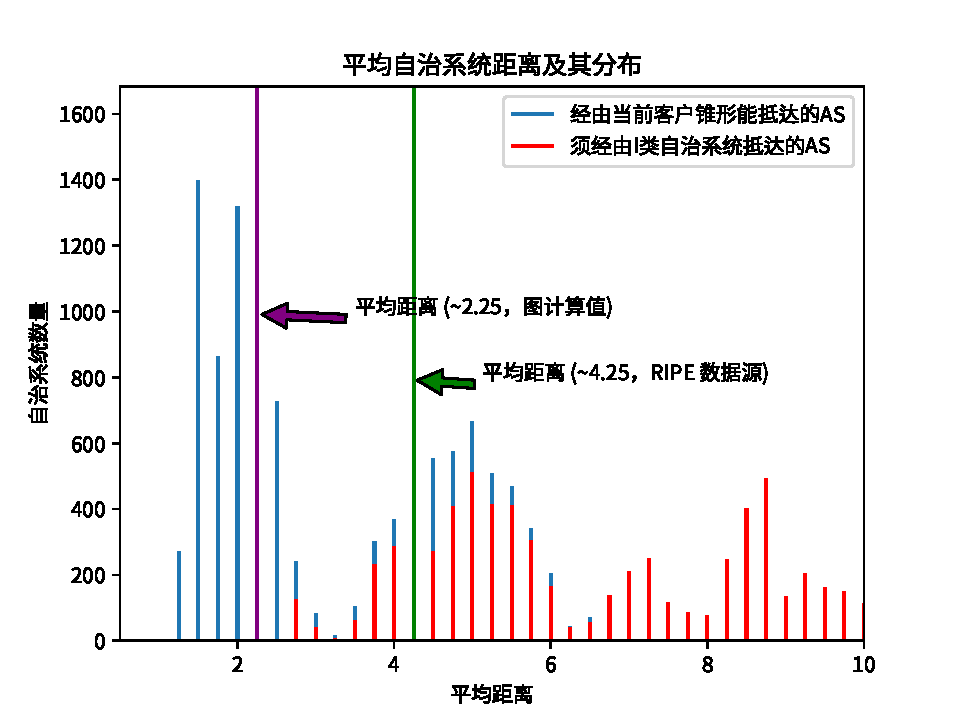
\includegraphics[width=0.85\linewidth]{chapter/c3_images/c3_as-distance.pdf}
    \caption{互联网中自治系统间的平均距离及其分布状况(RIPE RIS 数据集)}
    \label{c3_as-distance}
\end{figure}

图网络所包含的数据量也是一个值得注意的问题,事实上,据2020年一项研究报告称,全球互连网的路由数量已超过 $10^6$ 条,因而由路由数据构造的图大小本身已经超出了一些图网络模型的计算能力,这也是一些研究放弃图网络模型转而使用其它方法的原因。

此外,大部分模型研究的是特定于互联网路由表的异常检测,然而一些社区维护的分布式网络的拓扑结构与此并不相似,这类分布式网络尚未有满足本研究要求的数据集。

因而,从现有路由数据集和分布式网络出发,构建一种图网络数据集的生成算法是很有必要的。

\subsection{研究贡献}

本章从路由协议的角度出发,提出了一种新的路由数据构图方法,能够有效地去除网络中的冗余边和干扰因素,从而降低图的稠密性,使其能够在一些基于嵌入的异常检测模型下获得更好的效果,最后还使用了一些基于图网络的指标和基准算法来评估数据集的有效性,证明了它能够反映出与一般路由数据集相近的特征。

\section{数据获取和图生成模型}

% 3 页

\subsection{数据来源}

先前的章节总结了常见的路由数据集在多样性和尺度上存在不适用于图网络的问题,因此本文将使用来自互联网和 DN42 两种分布式网路的数据。

其中互联网的路由数据来源于 RIPE RIS 的公开数据集\citing{ripe2021routing},它将经过更多的处理步骤以解决数据规模和冗余数据等问题。而 DN42 则是一个去中心化的的实验性社区网络,它的数据集来源于 DN42 全球路由收集器(Global Route Collector)的数据\citing{dn42us}。与 RIPE RIS 相似地,DN42 GRC \citing{dn422022mrt}也提供了 DN42 下几乎全部的路由信息。 

不同的是,由于 DN42 相对于管理规则更为严格的互联网而言具有更加扁平的结构\citing{dn42us},因而具有更强的分布式特点,同时由于其实验性的定位,会更频繁地发生 BGP 路由的异常,甚至能够合规地在一定范围内制造这样的异常以供研究用途,\citing{tsai2022design} 因此本文在互联网之外还使用了这一数据集,在后续的研究中也会借助 DN42 作为一些算法的案例分析。

如表格 \ref{dataset-compare} 所示,本研究采集了相近时间的来自两种网络的数据,并总结了以上两种数据来源的不同之处,可见它们在数据规模、复杂度和结构特点上都有所不同,本研究尝试通过两类截然不同的网络结构的数据集来研究模型在面对不同结构的网络路由上,是否能保持一致的准确度,以便测试模型的泛用性。

\begin{table}
    \caption{两种数据集的参数对比}
    \begin{tabular}{p{0.2\linewidth}p{0.3\linewidth}p{0.3\linewidth}}
        \toprule
                       & \textbf{RIPE RIS}                                & \textbf{DN42 GRC}              \\
        \midrule
        宣告的IP前缀 \newline(IPv4) & $\sim$1,000,000                                  & $\sim$800                      \\
        宣告的IP前缀 \newline(IPv6) & $\sim$170,000                                    & $\sim$700                      \\
        可观测到的自治系统      & $\sim$70,000                                     & $\sim$500                      \\
        更新频率           & 8 小时 (全量),                     \newline5 分钟 (增量) & 10 分钟 (1周内), \newline1 天 (一周外) \\
        网络关系与拓扑        & 对等+非对等                                           & (几乎完全)双向非对等                    \\
        \midrule
        本文使用           & 性能评估                                             & 对照分析                           \\
        \bottomrule
    \end{tabular}
    \label{dataset-compare}
\end{table}

路由收集器提供的数据大多使用 MRT 格式,它能够完整地记录路由表中的多种路由信息,在本章节的研究中,MRT 文件中的路由将在数据的预处理阶段被导出,其中的自治系统路径和社区属性等信息是以图\ref{c3_data-struct}中的形式被保存在层次性的数据结构中,以便于后续将拓扑信息和其它属性分离开来。

\begin{figure}[h]
    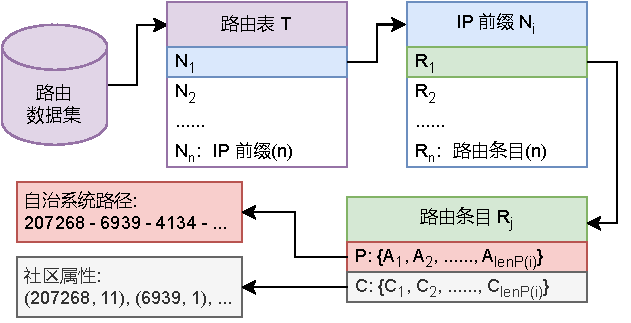
\includegraphics[width=0.7\linewidth]{chapter/c3_images/c3_data-struct.pdf}
    \caption{图网络路由数据集的组成结构,依层次为:路由数据集、路由表、网络前缀、路由及其包含的路径和社区属性}
    \label{c3_data-struct}
\end{figure}

\subsection{基于自治系统逻辑拓扑关系的图网络数据构建}

\subsubsection{层次结构分析}

\begin{figure}[h]
    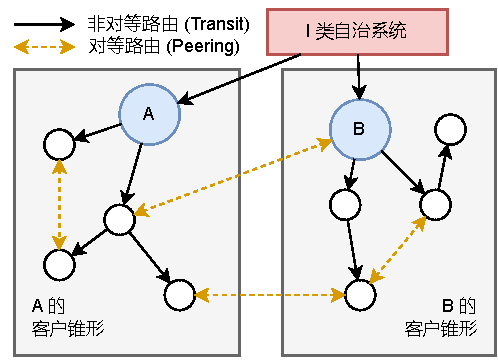
\includegraphics[width=0.6\linewidth]{chapter/c3_images/c3_dataset-layers.pdf}
    \caption{路由数据集的层次分解。由 A 和 B 建立的两个客户锥形之间存在的对等路由}
    \label{c3_dataset-layers}
\end{figure}

图 \ref{c3_as-distance} 的结果能够反映出,广域网络的一些连边事实上并不在路由信息的传递中扮演作用,这导致了完全通过网络路由数据集构建的图网络与真实路由系统的运作模式不一致,例如图中的平均自治系统长度的差异,而这些差异最终都将体现在模型的运行效果上。因而,为了实现下游模型训练效果的优化,需要从广域网络路由协议的角度去分析这些在路由过程中不扮演消息传递角色的路由,并将其从构造的图中去除。

通过对广域网路由模型的分析,广域网络的路由可以被抽象为一个类树状结构加上一些随机噪声连边,这种现象能够通过自治系统的互联模式很好的解释。如图 \ref{c3_dataset-layers} 所示,由于互联网络是由非对等互联路由和对等互联路由共同构成,前者具有一定的层次性,因而形成一种类树状结构;而后者则存在一定的无序性,因此能够随机地连接网络中的节点。由于对等路由仅仅在直接连接的自治系统之间交换路由,并不会传递其它自治系统的路由,因此这部分的路由在用于异常检测上时能够被移除而不影响异常检测的效果。

为了验证上述猜想,首先在图上定义对等路由:

对于一个路由表${R_i}$,某两个节点 $V_a$ 和 $V_b$ 的之间的路由$R_p$是自治系统长度为 1 的路由,假设其连边为 $E_p$,则它是对等(Peering)路由,当且仅当路由表${R_i}$的任意路由 $R_k$ 中不包含长度大于1,且路径末端为连边 $E_p$ 的自治系统路径。或者以公式\ref{peering_route}的方式表示:
\begin{equation} \label{peering_route}
R_p = \{P: \{E_p<V_a, V_b>\} \}, 
\forall R_k \in \{R_i\} \parallel len(P_k) \geq 1, E_p \neq last(P_k \in R_k)
\end{equation}

随后,为了研究现有数据集中的路由类型的分布状况,本研究使用了 RIPE RIS 和 DN42 在 2022年12月的数据集,对数据内节点介数中心度与它们的对等/非对等(Peering/Transit)路由的数量做出了统计和对比。实验结果如图 \ref{c3_route-centrality} 所示,可以从图中发现,互联网的非对等路由更具结构性,越具有中心度的节点,将具有越高的非对等路由,而对等路由则在大部分节点上呈现出随机的分布;作为对照,DN42 这类分布式网络由于大部分节点间完全通过双向非对等路由的形式进行路由交换,在路由数量与其介数中心度的关联上并没有互联网数据集密切。

\begin{figure}[h]
    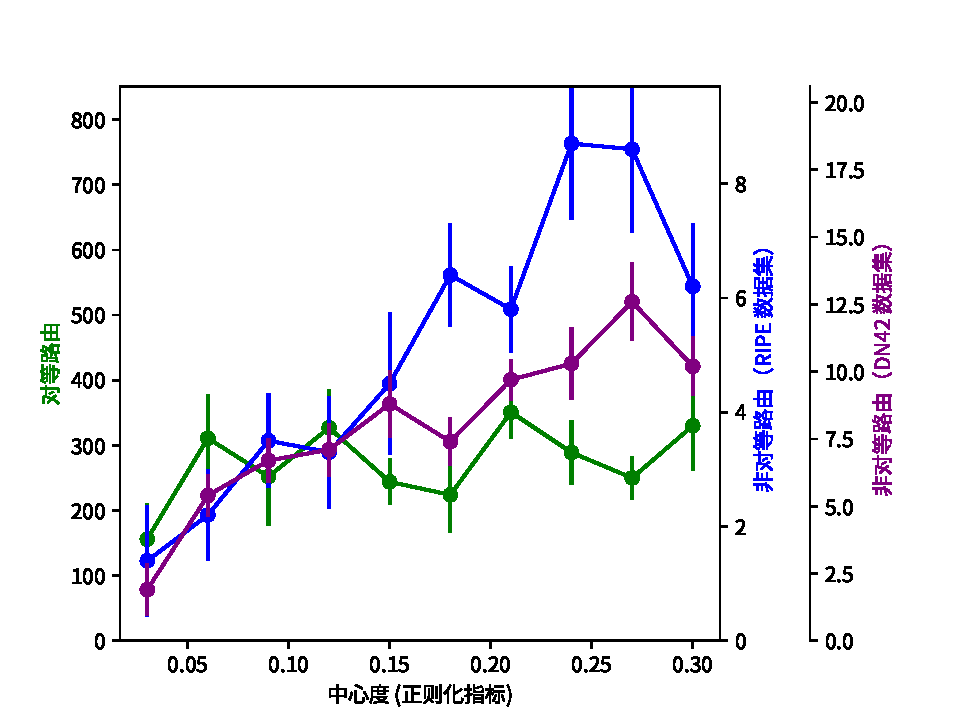
\includegraphics[width=0.9\linewidth]{chapter/c3_images/c3_route-centrality.pdf}
    \caption{路由数据集上对等/非对等(Peering/Transit)路由的数量与中心度的关联}
    \label{c3_route-centrality}
\end{figure}

假如去除路由系统中的对等连边,是否会有度为0的孤立节点产生是另一个因此出现的问题。根据路由条目沿非对等路由传播的定义,某个节点 $V_a$ 与 网络中任一节点互通,且并非通过对等方式互通(即 $d(V_a)\neq n-1$),则$V_a$与任一I类自治系统应当存在非对等路由关系,而根据I类自治系统的定义,没有任何节点向它们提供非对等路由,因此它必然存在一条通往I类自治系统的非对等路由。通过以上方式,能够证明,所有能够访问全部广域网的节点,要么与其余全部节点存在对等路由,要么存在至少一条可进入数据集的非对等路由。

% 对于自治系统节点 $V_a$,而言,设子图区域 $G_z = <\{V - V_a, E - E_a\}>$,其中 $E_a = \{ \forall E_k(V_{from}, V_{to}) \in E, if (V_{from} = V_a \parallel V_{to} = V_a ) \}$。假设 $V_a$ 不存在 Transit 路由,对于 $V_a$ 的临接节点集 $V_{nei}$,一定存在 $V_{nei} \leftrightarrow V_a $,即路由双向可达,由于 Peering 路由长度一定为 1,则对于 $V_a$ 的非临接节点集 $V - V_{nei}$ 一定在 $G_z$ 上存在一条通向 $V_a$ 的 Transit 路由,为了保证 $V_a$ 一定在 $V_{sample} \in V - V_a \in G_z$ 为起点的采样数据集中出现,即 $E\{P(V_a \rightarrow V_{sample})\} = 1$,要么 $V_{nei} =V - V_a$,要么 $V_a$ 存在至少一条 Transit 路由。

事实上,上述区域 $G_z$ 被称为DFZ(Default-Free Zone)区域,其被定义为拥有全部广域网路由的自治系统路由器集合。即使对等路由在实际网络中存在流量交换的意义,在此场景下仍然能够将其去除从而不影响图网络整体在异常检测上表现出的结构性。

\subsubsection{图生成算法}

在验证了上述假设的条件下,对路由数据的处理问题转化为了如何在现有的数据中提取并去除对等路由。

在此基础上,路由数据集的图生成算法定义如表 \ref{algo-datagen-topo} 所示。该算法能够通过上述方法去除没有对异常检测存在意义的对等互联路径,从而输出一张更具结构性特征的广域网路由拓扑图,从而达到降低网络复杂度、稠密度的效果。

\begin{algorithm}[H]
    \KwData{输入路由集合 \{$R_i$\} 和预先定义的I类ISP 表 $V_{t1}$}
    \KwResult{输出一份由此数据生成的数据集}
    初始化图网络:
    $G<V=\{\},E=\{\}>$\;
    提取路由路径:
    $\{P_i \in R_i\}$\;
    初始图网络生成:
    \For{$\{V_a, E_{ab}, V_b\} \in P_i$}{
    $G<V+=\{V_a, V_b\},E+={E_{ab}}>$
    }
    \For{每个非I类自治系统的节点$V_i \notin V_{t1}$,检查它们的连接 $e_i$:}{
        \If{$e_i$ 满足对等路由的条件}{
            从图中删除它: $G<V, E=E-e_i>$
        }
    }
    输出网络 $G$\;
    \caption{基于逻辑拓扑关系的路由图网络生成算法}
    \label{algo-datagen-topo}
\end{algorithm}

\subsection{基于自治系统路由相似度度量的图网络数据构建}

除了直接使用数据集中的路由数据进行图的拓扑构建外,还能使用原数据的节点相似度度量对图进行构建。这是对于过于冗余的原数据集的另一种利用方法,该方法将其转换为节点间路由度量的带权图,这能够将原本的路由拓扑图变得稀疏化,同时将冗余数据转化为正则化的指标。

虽然介数中心度在反映路由中心度上更具优势,但它的计算复杂度在面对互联网数据集的规模(>5000万条连边)的情况下过高,而在图网络中,基于余弦相似度的节点表征方法相比而言更加实际,它通过采样节点的邻居信息并实现对节点之间的相似度度量,并更加快速,适合使用在数据集的处理上。它的定义如公式 \ref{cos_dist} 所示。
\begin{equation} \label{cos_dist}
d_{cos}(V_A,V_B) = \frac{\Sigma_{nei} V_i^A V_i^B}{\sqrt{\Sigma_{nei} (V_i^A)^2} \sqrt{\Sigma_{nei} (V_i^B)^2}}
\end{equation}
% 公式

根据上述定义,使用以下算法利用相似度度量对原始数据集进行处理:

% 构图算法表格

\begin{algorithm}[H]
    \KwData{输入路由集合 $\{R_i\}$}
    \KwResult{输出一份由此数据生成的数据集}
    初始化图网络:
    $G<V=\{\},E=\{\}>$\;
    \For{每条路径 $\{P_i \in R_i\}$}{
        \For{路径上的相邻两个自治系统 $(V_a, V_b) \in P_i$}{
            对边赋权重:$e(V_a, V_b) += d_{cos}(V_a, V_b)$
        }
    }
    \For{图 $G$ 中的每个顶点 $\{V_i \in V \in G\}$}{
        \For{顶点上的每条边 $(V_a, V_b) \in E(V_i)$}{
            \eIf{进行 top-k 计算:$topk(E(V_a, V_b))$}{
                保留边 $E(V_a, V_b)$ \;
            }
            {
                删除边 $E(V_a, V_b)$ \;
            }
        }
    }
    输出网络 $G$\;
    \caption{基于路由相似度度量的路由图网络生成算法}
    \label{algo-datagen-sim}
\end{algorithm}

如表 \ref{algo-datagen-sim} 所示的算法描述,在获取数据集后,对路径上每一对自治系统节点间的相似度进行余弦相似度计算,将其作为邻接矩阵的权值。对于生成的临接矩阵,它是一个全连接的完全图,使用每节点 topk 权值的平均值作为分界值,从而将其变为更加稀疏的图网络。

\section{实验及分析}
% 4-5 页

在本章节的实验环节,首先需要比较的是输入的数据集在参数规模上的横向差异,这对后续异常检测任务的效果差异的分析上具有作用;其次,由于本章所述方法是对数据集中图网络结构的变换,本文还将针对此方法输入和输出图网络的参数进行纵向对比,以初步分析所述方法在去除冗余边集和降低邻接矩阵稠密度上的效果。

在数字特征上反映出的优化效果仅反映在时间维度上,因而本文在接下来的对比实验中,采用了多种基于不同方法的模型以评估图网络生成算法在异常检测任务中的提升效果,从而评估算法在何种程度上保持和聚合数据集中原有拓扑特征;随后在案例分析中,本研究通过仿真的实验环境评估了两种方法在改善模型检测效果上的提升。

\subsection{数据集概述}

对于本章节提出的模型而言,它的性能不仅取决于是否能够在具有较强结构化拓扑特征的互联网数据集上取得良好的效果,还应当考虑其横向泛化特性,即是否能够适用于并不明显具有结构化拓扑特征的网络。先前章节提到了 DN42 是一类分布式网络,它相比由 IANA 管理的网络而言更具松散的结构而具有更少的层次性,适合用于本章节的实验部分。

在模型参数分析部分,由于未涉及到预设的异常参考值,本文采用了最近的来自两个分布式网络的路由数据,它们分别是采用了来自 RIPE RIS 的三个较近时间点的数据集和来自 DN42 的一个较近时间点的数据集,均采用 MRT 格式。相应的数据统计信息如表格 \ref{c3_data_input} 所示。

\begin{table}
    \caption{作为输入的路由数据集的统计信息}
    \begin{tabular}{lcccccccc}
        \toprule
        指标/数据集 & RIPE.2022.10 & RIPE.2022.11 & RIPE.2022.12 & DN42.2022.12 \\
        \midrule
        路由总数   & 10,068,040   & 10,072,615   & 10,165,549   & 82,664       \\
        前缀总数   & 103,162      & 104,265      & 104,523      & 716          \\
        \midrule
        节点总数   & 75,105       & 75,363       & 75,442       & 557          \\
        连边总数   & 2,228,343    & 2,230,203    & 2,246,004    & 2,756        \\
        \bottomrule
    \end{tabular}
    \label{c3_data_input}
\end{table}

在后续参数的使用上,对于基于相似度的构图方法的 k 值,本文从基于逻辑拓扑关系的构图结果中获取图网络的平均度数作为对应的值,具体的来讲,对于 RIPE 的几个数据集,它们的值为 4.35,对于 DN42 的数据集而言,它的值为 9.62,与基于 RIPE RIS 和 DN42 原始数据的估计是相近的。

% 数据量,表格 

\subsection{参数分析}

图网络参数是一个需要被首先考虑的问题,本文通过对上述三组来自 RIPE RIS 数据的输出连边数量及下降比例分析,总结出如表 \ref{c3_data_arg} 所示的结果。

从表 \ref{c3_data_arg} 中基于拓扑的模型的统计数据可以发现,该方法在对降低具有较多对等路由的网络连边数量具有较大的作用,这是该方法的原理所决定的,对于 RIPE 数据集而言,模型最大能够降低约 17\% 的无效连边数,其数量级约为 $10^6$ 左右,这在基于消息传递的多层图网络模型的嵌入效果和计算复杂度上会反映为较大的差异。

在 DN42 分布式网络数据集上,基于拓扑结构的构图算法并不能够取得与互联网数据集一致的边集优化效果,这一点可以从先前章节对 DN42 网络结构的概述中得到解释:具有实验性质的网络通常不具备较高的层次性,因而也存在较少的对等路由,对于此种广域网络系统上的路由异常检测需要更好的优化方案。

在基于相似度的图生成模型上,由于设定的参数 k 对边集大小具有控制作用,因而此处的数值对比意义不大,仅反映对应 k 值在路由数据集上的对应结果规模。在异常检测模型的实际运行中,需要兼顾计算效率和运算性能以确定最优的 k 值。

\begin{table}
    \caption{输入与输出的图网络参数对比}
    \begin{tabular}{llcccccccc}
        \toprule
        算法                     & 指标/数据集 & RIPE.2022.10 & RIPE.2022.11 & RIPE.2022.12 & DN42.2022.12 \\
        \midrule
        \multirow{2}{*}{基于拓扑}  & 输出连边 & 1,847,296    & 1,857,759    & 1,866,429    & 2,552        \\
                               & 下降比率   & 17.1\%       & 16.7\%       & 16.9\%       & 7.4\%        \\
        \midrule
        \multirow{2}{*}{基于相似度} & 输出连边 & 2,092,414    & 2,065,167    & 2,091,029    & 2,599        \\
                               & 下降比率   & 6.1\%        & 7.4\%        & 6.9\%        & 5.7\%        \\
        \bottomrule
    \end{tabular}
    \label{c3_data_arg}
\end{table}

\subsection{对比实验}

\subsubsection{分析指标}

% 跑一个模型,随机选取一系列路径,看对同一个新增路径数据的前后结果是否在同一个 rank 上。
为了检验数据集是否在拓扑特征上与处理前一致,本章节将已知的网络路由异常数据集提供给多个无监督的图嵌入模型,并分析在路由异常事件间的异常路由检出的准确度和 F1 值。具体地,本实验选择了 HOPE,DeepWalk,GraphSAGE 三种图网络嵌入的基线算法进行衡量,以标准化误差 0.5 作为异常阈值。

在数据集的选取上,对比实验选择了 RIPE RIS 于 2010、2017、2022 三个时间段上具有已知异常路由异常标记的数据集,使用异常发生前一天作为基准数据训练模型,并将路由异常开始后的流式路由更新输入到模型以获取路由异常检测的输出值作为对比。

\subsubsection{实验结果}

此实验采用了上述基线模型来评估图生成算法降低冗余和无效连边的性能,表 \ref{c3_s3tab} 报告了在不同模型下的异常检测结果,从中可以得到下列的发现:

\begin{enumerate}
    \item 相比于原始数据而言,基于拓扑和基于相似度的图构建方法与各基线模型的配合在大部分场景下能够取得异常检测结果的改善,这意味着本章所提出的模型达到了预期的效果。
    \item 基于拓扑的构图模型在总体上优于本实验中设定数值的基于相似度的构图模型,本研究将其归结于两种原因:
          \begin{enumerate}
              \item 其一是尽管基于相似度的构图方法能够通过对节点特征相似度的 topk 的方式降低原始数据在图上的稠密度,但它实质上并没有在根本上移除无效边集,因而在输出的图网络中引入了噪声。
              \item 其二是基于相似度的构图方法的效果完全依赖于 top-k 中确定的 k 值,而对于原始数据实际组成的图网络而言,节点的连边数量将会根据节点的重要程度产生不同的权重。
          \end{enumerate}
    \item 对于基于拓扑的图构建方法而言,总体上各异常检测模型在更具结构化、邻接节点和路由关系更加复杂的互联网路由数据集(RIPE 数据集)能够取得更好的效果,这是符合本研究的参数分析章节的预期的结果。
    \item 基于相似度的构图模型上在使用类似 DN42 的分布式网络数据集上存在性能不佳的问题,其中的一种可能原因是,管理松散、相互连接从而具有较少层次结构的分布式网络的节点之间的相似度距离会更加接近。
\end{enumerate}

\begin{table}
    \caption{对比实验结果}
    \begin{tabular}{lcccccccc}
        \toprule
                        & \multicolumn{2}{l}{RIPE.2010} & \multicolumn{2}{l}{RIPE.2017} & \multicolumn{2}{l}{RIPE.2022} & \multicolumn{2}{l}{DN42.2022}                                                                     \\ \cmidrule(lr){2-3} \cmidrule(lr){4-5} \cmidrule(lr){6-7} \cmidrule(lr){8-9}
        模型              & Acc.                          & F-1                           & Acc.                          & F-1                           & Acc.           & F-1            & Acc.           & F-1            \\ \midrule
        原始数据                                                                                                                                                                                                                \\
        \quad HOPE      & 0.712                         & 0.698                         & 0.708                         & 0.682                         & 0.709          & 0.688          & 0.692          & 0.671          \\
        \quad DeepWalk  & 0.768                         & 0.770                         & 0.754                         & 0.741                         & 0.750          & 0.757          & 0.751          & 0.755          \\
        \quad GraphSAGE & 0.793                         & 0.820                         & 0.815                         & 0.808                         & 0.784          & 0.814          & 0.807          & 0.801          \\ \midrule
        基于拓扑的构图模型                                                                                                                                                                                                           \\
        \quad HOPE      & 0.761                         & 0.754                         & 0.734                         & 0.721                         & 0.770          & 0.724          & 0.748          & 0.727          \\
        \quad DeepWalk  & 0.794                         & 0.784                         & 0.791                         & 0.786                         & 0.809          & 0.802          & 0.771          & 0.776          \\
        \quad GraphSAGE & \textbf{0.835}                & 0.824                         & \textbf{0.843}                & \textbf{0.821}                & \textbf{0.830} & \textbf{0.840} & \textbf{0.809} & \textbf{0.813} \\ \midrule
        基于相似度的构图模型                                                                                                                                                                                                          \\
        \quad HOPE      & 0.705                         & 0.703                         & 0.721                         & 0.715                         & 0.722          & 0.711          & 0.682          & 0.673
        \\
        \quad DeepWalk  & 0.780                         & 0.767                         & 0.778                         & 0.760                         & 0.762          & 0.752          & 0.759          & 0.770          \\
        \quad GraphSAGE & 0.823                         & \textbf{0.830}                & 0.820                         & 0.810                         & 0.812          & 0.826          & 0.801          & 0.807
        \\
        \bottomrule
    \end{tabular}
    \label{c3_s3tab}
\end{table}

\subsection{案例分析}

\subsubsection{实验方法}

为了确定模型性能的改善是由于图构建时采用的算法,本章基于 DN42 平台构建了仿真的测试环境,试图通过案例分析的方式确定算法的有效性。

如图 \ref{c3_case-flow} 所示,作为实验环境的初始化,节点 A(AS4242421331) 被接入到 DN42 网络中,并将其与 B(AS4201271332) 构成对等路由关系,其中 C(AS4242421331) 是 A 和 B 的共同 Transit 提供者,这是一个用于验证本章所述算法正确性的最小可操作场景。通过节点 A 向 DN42 的路由收集器发起路由反馈会话,并维持正常的网络路由一段时间,正常的路由表能够被 GRC 收集并生成数据集文件。

在随后的实验步骤中,节点 A 通过更长前缀的方式劫持节点 B 的路由,意图将通往该网络的流量劫持至节点 A 所控制的网络中。该行为将被网络自身及其各阶邻居通告给 GRC,随后 GRC 将以更新文件的形式将包含异常路由的路由表生成出来。

\begin{figure}[h]
    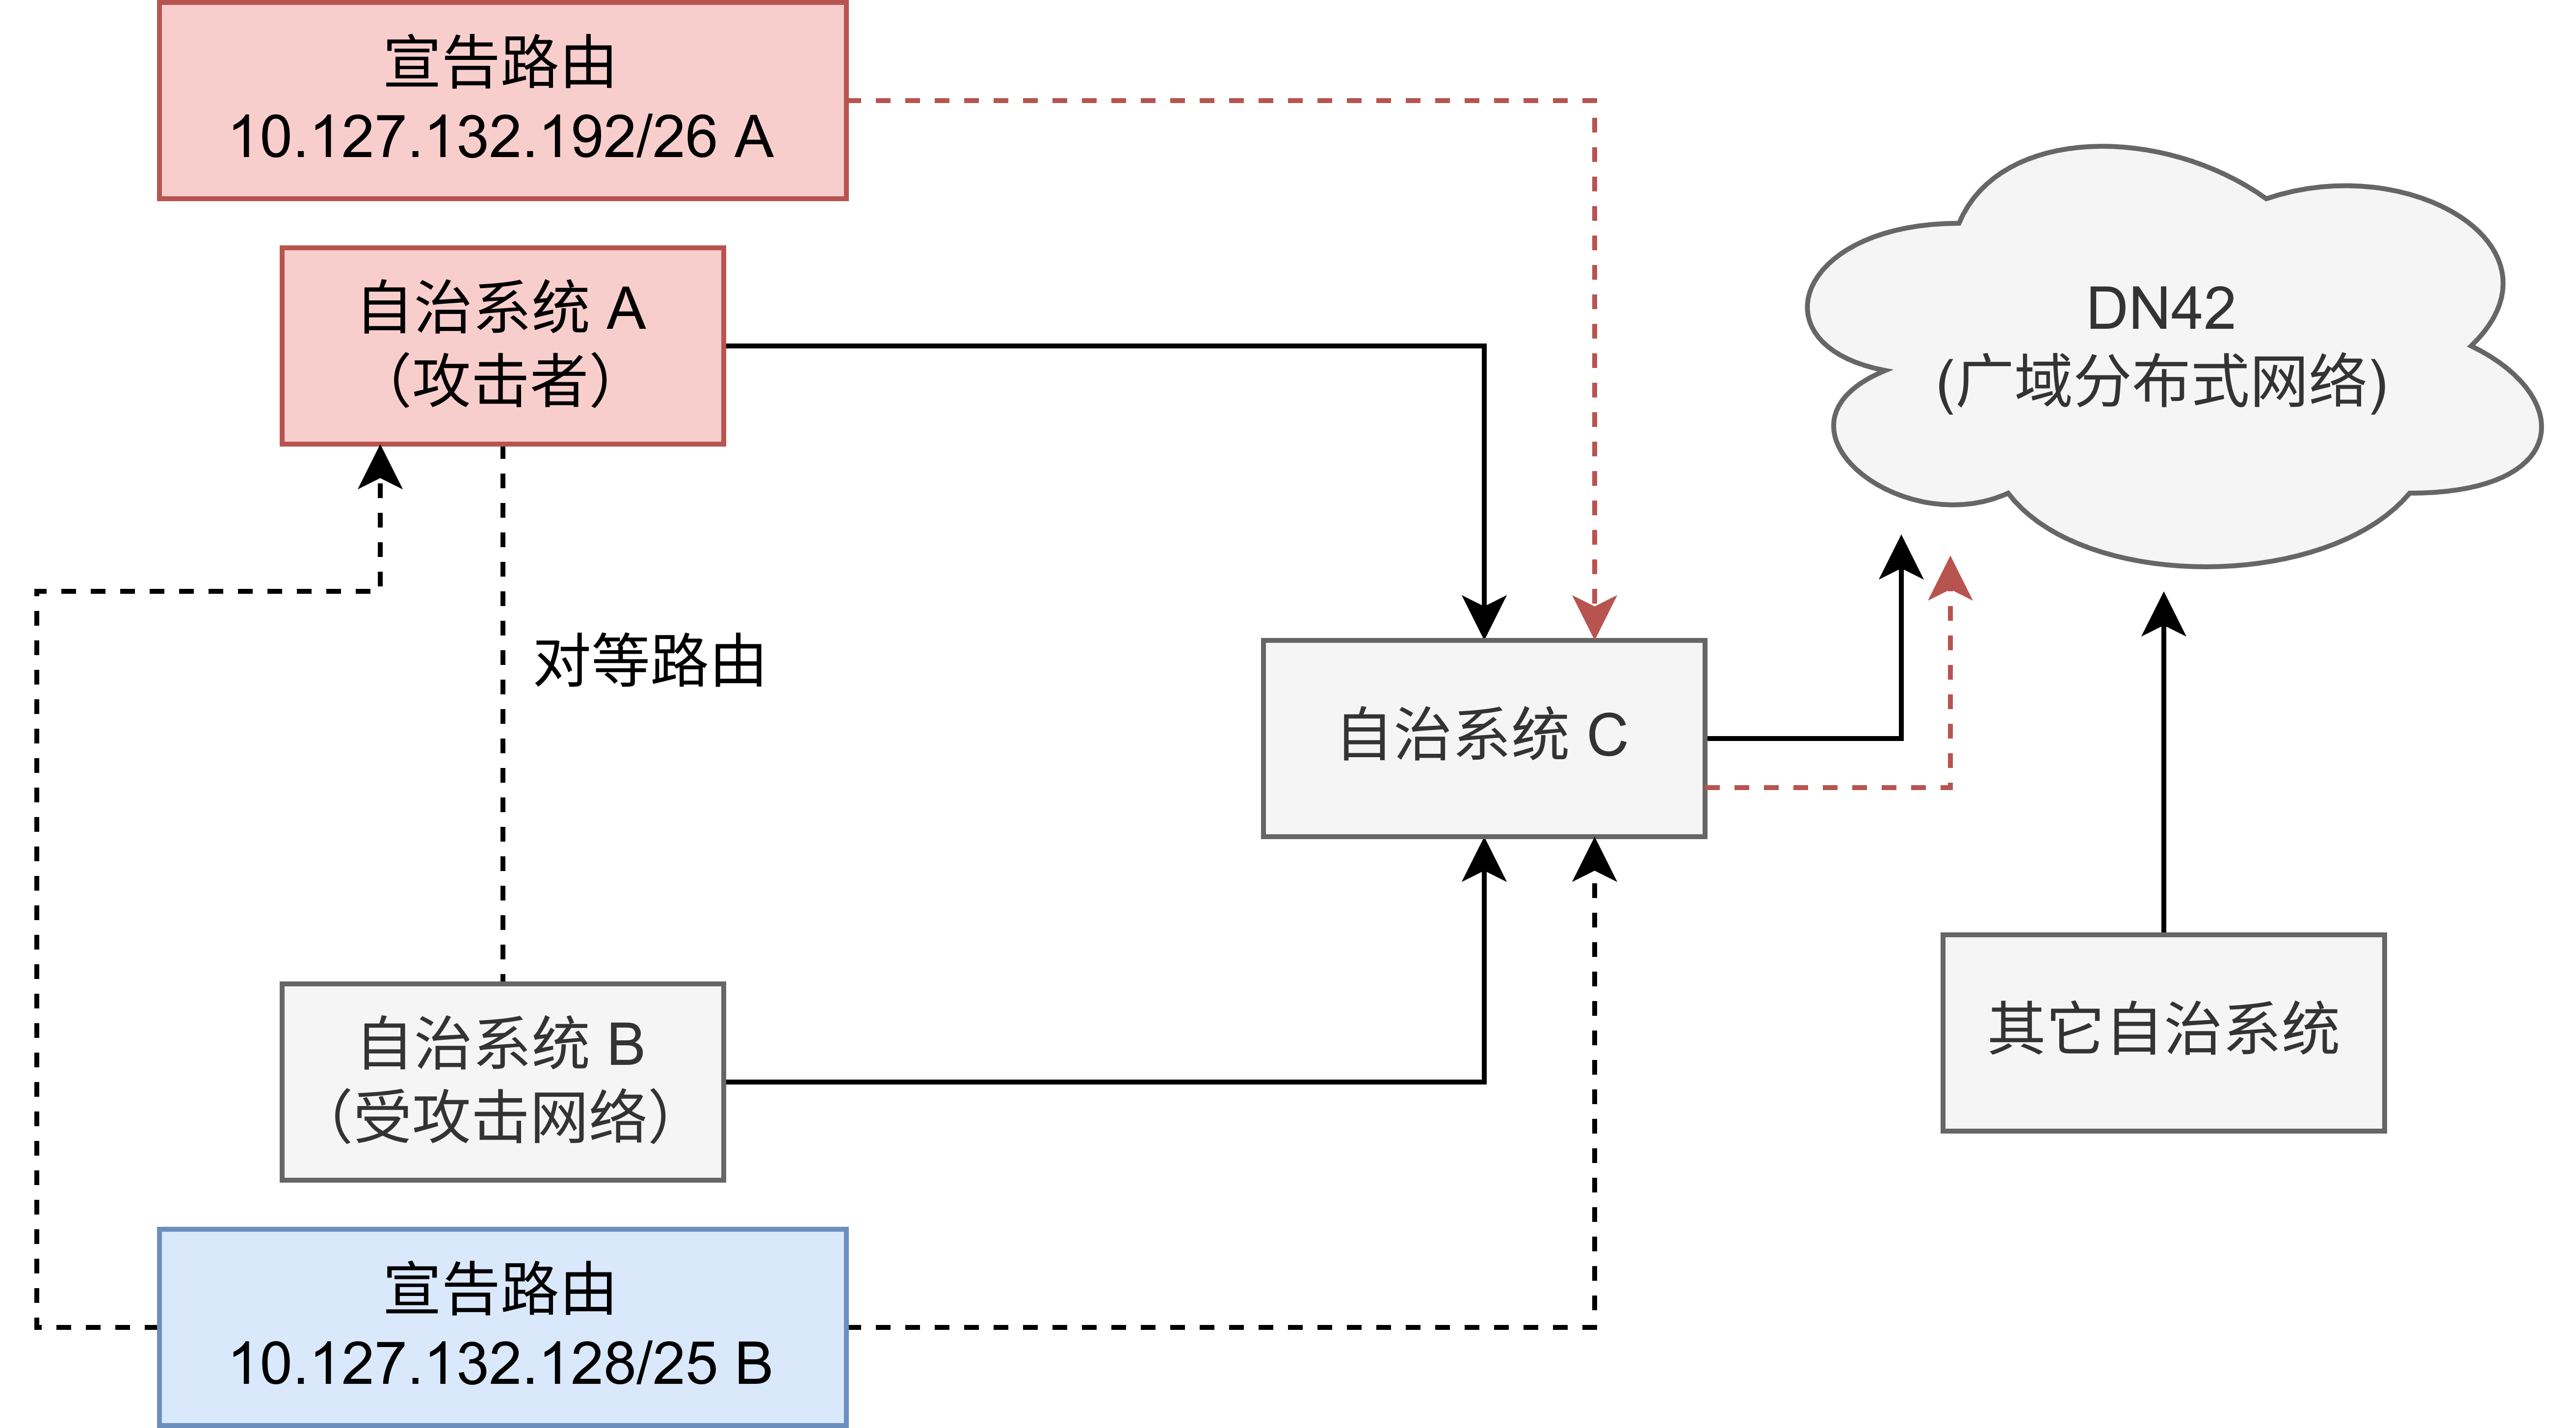
\includegraphics[width=0.7\linewidth]{chapter/c3_images/c3_case_flow.png}
    \caption{案例分析实验流程}
    \label{c3_case-flow}
\end{figure}

上述模型将以这两个文件作为输入,使用 GraphSAGE 算法模型进行嵌入并输出异常分数,从而判断本章所提出的算法对无效和冗余路由的去除效果,及对嵌入结果的影响。由于在此实验中,异常路由是已知的,因而可以从数据集中获取所有包含异常的路由样本,并将其送入模型进行异常检测。

基于对比实验的效果及在图构建算法设计上的规则,预期的结果是,使用原有数据集构成的路径的模型将在所有异常样本中取得相对更低的分数,而使用基于结构特征的构图方式的模型将在所有样本中取得相对更高的分数在,这是由于如图 \ref{c3_case-flow} 所示,在不去除自治系统 A 和自治系统 B 之间的对等路由的状况下,由原数据产生的图网络将包含 A、B 之间的连边,从而将 A、B 两个节点间的嵌入相似度拉近,进而影响到异常检测的分数。

\subsubsection{实验结果}

对于基于两种构图方式的所有异常路由样本的异常分数输出如图 \ref{c3_case-score} 所示。可见两种模型在异常样本的输出上与预期基本符合,与原始数据集相比在相同模型的分数输出上均具有提升。其中,基于结构特征的构图方式总体上对异常路由的预测效果提升最大(异常分数提升约 30\%),这反映出了基于结构特征的构图方式达到了相对而言更好的去除冗余路由的效果,而基于相似度的构图方式也相对于完全使用原始数据构图的方法在异常检测分数上提高了约 18\%,此结果展现出了,即使在不去除原始拓扑中的冗余路由的情况下,适当降低输入图网络的邻接矩阵稠密度同样能够改善模型的检测效果。

\begin{figure}[h]
    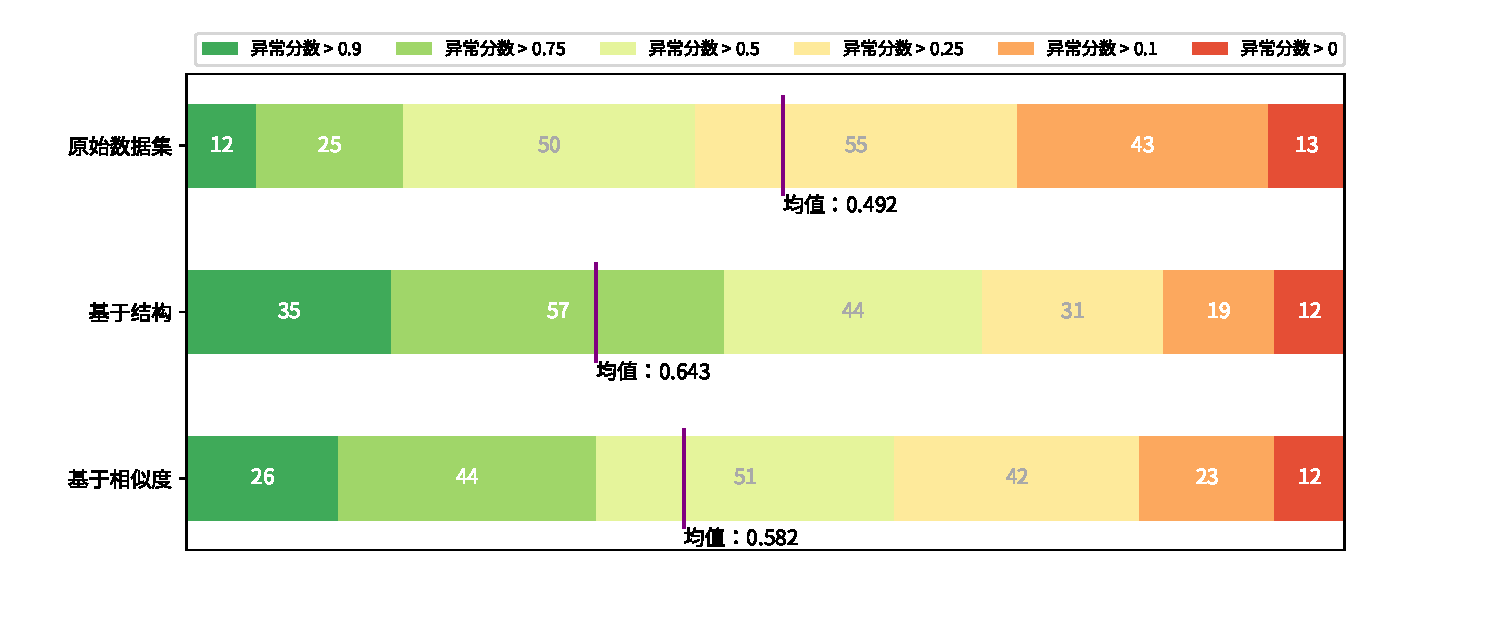
\includegraphics[width=\linewidth]{chapter/c3_images/c3_case-score.pdf}
    \caption{两种模型在异常路由样本下的输出分数}
    \label{c3_case-score}
\end{figure}

\section{本章小结}

本章主要针对海量路由数据集提出了一种图数据生成算法。在 3.1 节,介绍了现有的广域网路由数据集,并分析了其中存在的问题及对图网络模型的影响。在 3.2 节,本文通过分析广域网络的拓扑结构特征,将路由数据集中的噪声通过一种基于客户锥形的方法分离出来,并设计出了两种不同方式的图生成算法框架。在 2.3 节,为了实证数据集的有效性,通过节点相似度和嵌入相似度的比较,本文使用一些常见的基线模型在该算法生成的数据集中进行了实验分析。